\section{Model}
\subsection{Sections}
Regardless of the Power Integrity issues, memories are organized so that each output data pin \texttt{DQ} is interleaved with \texttt{VDDQ} and \texttt{VSSQ} power pins as in \autoref{fig:pin-layout} to help the receiver recognizing the data which may be distorted at such high speeds.
\begin{figure}[htbp]
	\center
	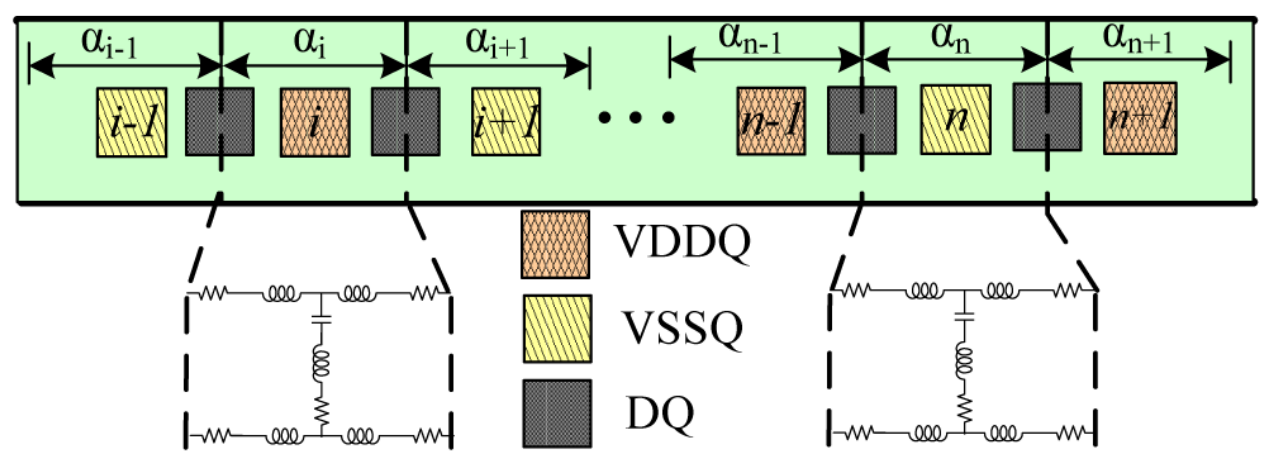
\includegraphics[width = \textwidth]{img/pin-layout}
	\caption{Pin layout of a memory chip}
	\label{fig:pin-layout}
\end{figure}

\autoref{fig:pin-layout} also shows how the memory can be subdivided in sections of length $\alpha_i$ which are not necessarily equal. Each section can be modeled with a two port device strucured as in \autoref{fig:tsection-model}.
\begin{figure}[htbp]
	\center
	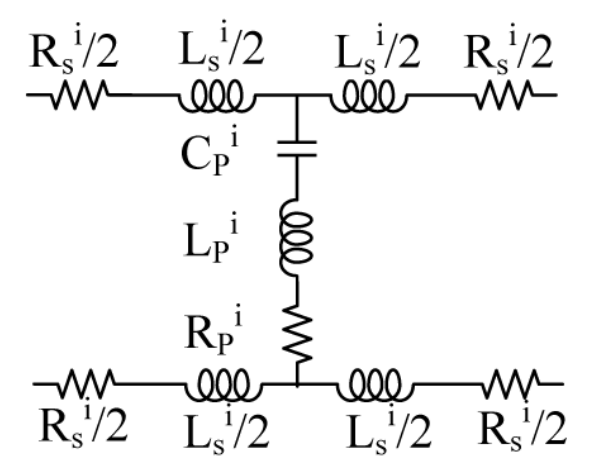
\includegraphics[width = 0.4\textwidth]{img/tsection-model}
	\caption{Model of a single section of a memory output}
	\label{fig:tsection-model}
\end{figure}

\subsection{Parameters}
\label{ssec:parameters}
Each section will thus have five characterizing parameters: $R^i_s$, $L^i_s$, $R^i_p$, $L^i_p$, $C^i_p$. These parameters depend on the overall Per-Unit-Length (PUL) parameters $R_s$, $L_s$, $R_p$, $L_p$, $C_p$ and the length of each section $\alpha_i$. Given this model, the objective is to fit a set of real measurements in order to infer the memory PUL parameters which, in turn, will determine each section's parameters.

This model can also account for the skin effect with a simple change, which is integrated in the final solution. Specifically, it is possible to split the PUL parameters $R_s$ and $R_p$ into $R_{s,\,dc}$, $R_{s,\,ac}$, $R_{p,\,dc}$ and $R_{p,\,ac}$. In order to map the PUL parameters to section-specific parameters it is possible to use:
\begin{align*}
    R^i_s &= \alpha_i \max\left(R_{s,\,dc},\, R_{s,\,ac}\sqrt{\omega}\right) \\
    L^i_s &= \alpha_i L_s \\
    R^i_p &= \frac{1}{\alpha_i} \max\left(R_{p,\,dc},\, R_{p,\,ac}\sqrt{\omega}\right) \\
    L^i_p &= \frac{1}{\alpha_i} L_p \\
    C^i_p &= \alpha_i C_p
\end{align*}

\subsection{Fitting}
\label{ssec:fitting}
The unknowns of the problem are the PUL parameters - section lengths are to be manually measured or retrieved from layout information. The measured quantity is the two port $Z$ matrix throughout a certain range of frequencies between two arbitrary ports of the device.

To be able to compare the real-world measurements to the simulated values we need to transform the device PUL parameters to its $Z$ matrix between the same two ports of the measurements. This procedure is discussed in \autoref{ssec:from-parameters-to-Z-matrix}.

The fitting process will thus be reduced to a multi-variable optimization process, where the input is a vector representing the PUL parameters and the evaluated function will be an error function - the distance between the model and physical device. In this case:
\begin{align*}
    U\left(\vec{p}\right) &= \sum_{i = 0}^N \left|| Z_s\left(\vec{p}, f_i\right) - Z_m(f_i) \right|| ^2
\end{align*}
where $\vec{p}$ is a vector representing the device PUL parameters, $N$ is the total number of measured frequencies, $f_i$ is the i-th measured frequency, $Z_s$ is the impedance matrix obtained from the simulation and $Z_m$ is the measured matrix.

\subsection{From PUL Parameters to Z Matrix}
\label{ssec:from-parameters-to-Z-matrix}
In the previously mentioned $U(\vec{p})$ formula it is necessary to compute $Z_s\left(\vec{p}, f_i\right)$, which means computing an impedance matrix between two fixed ports of the device starting from its PUL parameters. The passages are as follows:
\begin{enumerate}
    \item Compute each section's parameters from PUL parameters as in \autoref{ssec:parameters}
    \item Compute each section's ABCD matrix with
    \begin{equation*}
        \text{ABCD} = \begin{bmatrix}
            1 + z_i y_i   & (z_i y_i + 2) z_i \\
            y_i           & 1 + z_i y_i
        \end{bmatrix}
    \end{equation*}
    where
    \begin{align*}
        z_i &= j \omega L_s^i + R_s^i \\
        y_i &= \frac{j \omega C_p^i}{1 + j\omega R_p^i C_p^i - \omega^2 L_p^i C_p^i}
    \end{align*}
    \item Divide the layout into three groups by cumulating ABCD matrices: before port 1 ($M_1 = \prod_{i = 0} ^ \text{P1} \text{ABCD}_i$), between port 1 and port 2 ($M_2 = \prod_{i = \text{P1}} ^ \text{P2} \text{ABCD}_i$) and after port 2 ($M_1 = \prod_{i = \text{P2}} ^ R \text{ABCD}_i$).

    \item Compute the $Y$ matrix with
    \begin{align*}
        Y(1, 1) &= \frac{M_1(2, 1)}{M_1(2, 2)} + \frac{M_2(2, 2)}{M_2(1, 2)} \\
        Y(1, 2) &= -\frac{1}{M_2(1, 2)} \\
        Y(2, 1) &= Y(1, 2) \\
        Y(2, 2) &= \frac{M_2(1, 1)}{M_2(1, 2)} + \frac{M_3(2, 1)}{M_3(1, 1)}
    \end{align*}
    \item Invert $Y$ to get the desired $Z$ matrix
\end{enumerate}

\subsection{Results}
After finding the best $\vec{p}$ that minimizes $U(\vec{p})$, the resulting PUL parameters are a good description of the physical device and the model error is limited. It is possible at this point to simulate a frequency sweep and compare the simulated model to its real world counterpart.
